\documentclass[11pt,a4paper]{article}

\usepackage{../../templates/style}

\begin{document}

\begin{problem}{Tile}{standard input}{standard output}{1 second}{16 megabytes}

วางกระเบื้องวงกลม $N$  ชิ้น แต่ละชิ้นมีรัศมีไม่เกิน $10$ หน่วยลงบนสนาม  โดยกระเบื้องชิ้นที่ $i$ มีจุดศูนย์กลางอยู่ที่พิกัด $(X_i , Y_i)$  ที่เป็นจำนวนเต็ม และมีรัศมี $R_i$ เราทราบว่าไม่มีกระเบื้องคู่ใดที่มีจุดศูนย์กลางเป็นจุดเดียวกัน

กระเบื้องสองชิ้น $i$ และ $j$ จะทับกันถ้า จุดศูนย์กลางอยู่ห่างกันน้อยกว่าผลรวมของรัศมี  นั่นคือ

$$(X_i – X_j)^2 + (Y_i –Y_j)^2 < (R_i + R_j)^2$$

\bigskip
\underline{\textbf{โจทย์}}  จงเขียนโปรแกรมเพื่อรับตำแหน่งและขนาดของกระเบื้องทั้งหมด จากนั้นให้คำนวณว่ามีกระเบื้องกี่คู่ที่ทับกัน

\InputFile

\textbf{บรรทัดแรก} รับค่าจำนวนเต็ม $N$ $(1 \leq N \leq 100\,000)$   

\textbf{บรรทัดที่ $2$ ถึง $N +1$} ในบรรทัดที่ $i+1$ จะระบุจำนวนเต็มสามค่า $X_i$  $Y_i$  $R_i$ เป็นข้อมูลของกระเบื้องแผ่นที่ $i$  $(-20\,000 \leq X_i \leq 20\,000;  -20\,000 \leq Y_i \leq 20\,000; 1 \leq R_i \leq 10)$  รับประกันว่าไม่มีคู่ของดัชนี $i$ และ $j$ ที่ไม่เท่ากันซึ่ง $X_i = X_j$ และ $Y_i = Y_j$   (นั่นคือ ไม่มีกระเบื้องสองอันใด ๆ ที่มีจุดศูนย์กลางเดียวกัน)

\OutputFile

\textbf{มีบรรทัดเดียว} เป็นจำนวนคู่ของกระเบื้องที่ทับกัน รับประกันว่าผลลัพธ์จะมีค่าไม่เกิน $2\,000\,000\,000$

\Examples

\begin{example}
\exmp{5
0 0 1
3 0 2
0 3 2
3 3 3
5 0 1}{4}%
\end{example}

\Note 

\begin{figure}[h]
\centering
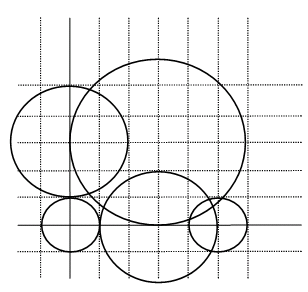
\includegraphics[width=0.7\textwidth]{../latex/img/1054/1054-1.png}
\caption{รูปประกอบตัวอย่างข้อมูลนำเข้า}
\end{figure}

\Scoring 

\textbf{ไม่น้อยกว่า 20\% ของข้อมูลชุดทดสอบ:} $N \leq 1\,000$

\Source

สอบปฏิบัติครั้งที่ 2 ค่ายคัดเลือกผู้แทนประเทศไทย ไปแข่งขันคอมพิวเตอร์โอลิมปิกระหว่างประเทศปี 2550 ค่ายที่ 1

\end{problem}

\end{document}